\chapter{The Standard Model of Particle Physics}

\section{The Standard Model}

The Standard Model (SM) of particle physics is a Lorentz-invariant quantum field theory (QFT) that describes the dynamics of elementary particles.  Three critical developments leading to the formation of the SM, as described by Steven Weinberg\cite{Weinberg:2004kv}, were the quark model proposed by Gell-Mann\cite{GellMann:1964nj} and Zweig\cite{Zweig:1964jf} in 1964, the idea of gauge symmetry by Yang and Mills\cite{Yang:1954ek} in 1954, and the notion of spontaneous symmetry breaking proposed by Goldstone\cite{Goldstone:1961eq} in 1961.  This ultimately led to the SM in its current form as a non-Abelian gauge theory with the symmetry group
\begin{equation}
	\label{equation:gaugesymmetry}
	G_{SM} = SU(3)_C \otimes SU(2)_L \otimes U(1)_Y
\end{equation}
where $SU(3)_C$ is responsible for strong interactions and $SU(2)_L \otimes U(1)_Y$ is responsible for unified electromagnetic and weak interactions, also known as electroweak interactions.

Associated with each of these symmetry groups is a set of massless spin-1 vector fields called gauge bosons.  These are listed in Table \ref{table:BosonFields} along with the associated charge or generator for that group.  There are eight such gauge bosons in $SU(3)_C$ called gluons $G_\mu^{1,...,8}$.  There are three gauge bosons $W_\mu^{1,2,3}$ in $SU(2)_L$ and one gauge boson $B_\mu$ in $U(1)_Y$.  The gauge bosons mediate the interactions between spin-1/2 fields $\psi$ called fermions.  At this point it's worth noting that the $W$ and $B$ gauge fields are not observable bosons, but are mixed by electroweak symmestry breaking to produce observable bosons.  The details of this will be covered in Section \ref{section:EWSB}.

There are twelve fermion fields which can be split into six lepton fields and six quark fields.  Both quarks and leptons are comprised of three generations.  For quarks there are three "up-type" quarks (up $u$, charm $c$, and top $t$) and three "down-type" quarks (down $d$, strange $s$, and bottom $b$).  The lepton fields are electron $e$, muon $\mu$, tau $\tau$, and three neutrino fields $\nu_e$, $\nu_\mu$, and $\nu_\tau$.  The fermion fields and their representations under $G_{SM}$ are listed in Table \ref{table:FermionTable}.  Each fermion field can be expressed in terms of left and right chirality fields, which are represented by a doublets $\psi_L$ in the left-handed case and singlets $\psi_R$ in the right-handed case with
\
\begin{eqnarray}
	\psi = \psi_R + \psi_L \\
	\psi_R = \frac{1}{2}(1+\gamma^5)\psi \\
	\psi_L = \frac{1}{2}(1-\gamma^5)\psi  
\end{eqnarray}

The SM also contains a complex scalar doublet field $\phi$ called the Higgs field in honor of Peter Higgs, who was among one of the physicists who proposed its existence in 1964 \cite{Higgs:1964pj}.  

\begin{table}[h!]
	\centering
	\caption{Boson fields in the SM}
	\begin{tabular}{|c|c|c|}
		\hline
		Symbol & Associated Charge & Symmetry group \\
		\hline
		\hline
		$B_\mu$ & weak hypercharge $Y$ & $U(1)_Y$\\
		\hline
		$G_{\mu}^{1,...,8}$ & color $C=(r,g,b)$ & $SU(3)_C$ \\
		\hline
		$W_{\mu}^{1,2,3}$ & weak isospin $T_3$ & $SU(2)_L$ \\
		\hline
	\end{tabular}
	\label{table:BosonFields}
\end{table}


%\begin{table}
%	\centering
%	\caption{Fermion fields in the SM.  }
%	\begin{tabular}{|c|c|c|}
%		\hline
%		Name & Symbol & \vbox{\hbox{\strut Representation under} \hbox{\strut $SU(3)_C, SU(2)_L, U(1)_Y$}} \\
%		\hline
%		\hline
%		Quarks & \vbox{\hbox{\strut($u_L$ $d_L$)} \hbox{\strut $u_{R}^\dagger$} \hbox{\strut $d_{R}^\dagger$}} & \vbox{\hbox{\strut (3, 2, $\frac{1}{6}$)}\hbox{\strut (3, 1, $-\frac{2}{3}$)}\hbox{\strut (3, 1, $\frac{1}{3}$)}} \\
%		\hline
%		Leptons & \vbox{\hbox{\strut($\nu$ $e_L$)}\hbox{\strut $e_{R}^\dagger$}} & \vbox{\hbox{\strut (3, 2, $-\frac{1}{2}$)} \hbox{\strut (1, 1, 1)}} \\
%		\hline
%	\end{tabular}
%	\label{table:FermionFields}
%\end{table}

\begin{table}
	\centering
	\caption{Fermions in the SM.  The first two numbers listed in the third column give the supermultiplet representation under $SU(3)_C$ and $SU(2)_L$ respectively.  A \textbf{1} means that it is not charged under that group and therefore will not couple to the associated force.  A \textbf{3} as the first number means that it has color charge and couples to the strong force.  A \textbf{2} for the second number means that it has weak isospin and couples to the weak force. The third number gives the value of the weak isospin.  Adjoint representation is specified by the presence of a bar over the number.}
	\begin{tabular}{|l|c|c|}
		\hline
		Name & Notation & \vbox{\hbox{\strut Representation under} \hbox{\strut $SU(3)_C \otimes SU(2)_L \otimes U(1)_Y$}} \\
		\hline
		\hline
		\vbox{\hbox{\strut Left-handed} \hbox{\strut quark doublet}} & 
		$
		\left(
		\begin{array}{c}
			u_L \\
			d_L \\
		\end{array}
		\right)
		$, 
		$
		\left(
		\begin{array}{c}
			c_L \\
			s_L \\
		\end{array}
		\right)
		$, 
		$
		\left(
		\begin{array}{c}
			t_L \\
			b_L \\
		\end{array}
		\right)
		$
		& (3, 2, $\frac{1}{6}$) \\
		\hline
		\vbox{\hbox{\strut Right-handed} \hbox{\strut up-type quark singlet}} & $u_R^\dagger$, $c_R^\dagger$, $b_R^\dagger$ & ($\bar{3}$, 1, -$\frac{2}{3}$) \\
		\hline
		\vbox{\hbox{\strut Right-handed} \hbox{\strut down-type quark singlet}} & $d_R^\dagger$, $s_R^\dagger$, $t_R^\dagger$ & ($\bar{3}$, 1, $\frac{1}{3}$) \\
		\hline
		\vbox{\hbox{\strut Left-handed} \hbox{\strut lepton doublet}} & 
		$
		\left(
		\begin{array}{c}
			\nu_{eL} \\
			e_L \\
		\end{array}
		\right)
		$, 
		$
		\left(
		\begin{array}{c}
			\nu_{\mu L} \\
			\mu_L \\
		\end{array}
		\right)
		$, 
		$
		\left(
		\begin{array}{c}
			\nu_{\tau L} \\
			\tau_L \\
		\end{array}
		\right)
		$
		& (1, 2, -$\frac{1}{2}$) \\
		\hline
		\vbox{\hbox{\strut Right-handed} \hbox{\strut charged lepton singlet}} & $e_R^\dagger$, $\mu_R^\dagger$, $\tau_R^\dagger$ & ($\bar{1}$, 1, 1) \\	
		\hline	
	\end{tabular}
\label{table:FermionTable}
\end{table}

The strong interaction is described by the theory of quantum chromodynamics (QCD).  The Lagrangian for the QCD interaction can be written as
\begin{equation}
	\mathcal{L}_{QCD} = \bar{\psi}(i\gamma^\mu D_\mu -m)\psi - \frac{1}{2}TrG_{\mu \nu}G^{\mu \nu}
	\label{equation:qcdlagrangian}
\end{equation}
where  
\begin{eqnarray}
	G_{\mu \nu} = \partial_\mu G_\nu - \partial_\nu G_\mu - ig_s[G_\mu , G_\nu] \\
	D_\mu = \partial_\mu - ig_sG_\mu
\end{eqnarray}
$g_s$ is related to the strong coupling constant, and $m$ is the fermion mass, which in this case must be a quark since they are the only fermions with color charge.

\section{Electroweak Symmetry Breaking} \label{section:EWSB}
A crucial feature of the SM is electroweak symmetry breaking.  The electroweak interaction, first proposed by Glashow, Weinberg, and Salam in the 60's, is the unified description of electromagnetic and weak interactions under the $SU(2)_L \otimes U(1)_Y$ symmetry.  The electromagnetic interaction is described by quantum electrodynamics (QED), which is an Abelian gauge theory under the $U(1)_{EM}$ symmetry group.  The gauge boson in QED is the photon and couples to electric charge $Q$. The QED Lagrangian is given by
\begin{equation}
	\mathcal{L}_{QED} = \bar{\psi}(i\gamma^\mu D_\mu -m)\psi - \frac{1}{4}F_{\mu \nu}F^{\mu \nu}
	\label{equation:qedlagrangian}
\end{equation}
where   
\begin{eqnarray}
	F_{\mu \nu} = \partial_\mu A_\nu - \partial_\nu A_\mu \\
	D_\mu = \partial_\mu + ieQA_\mu
\end{eqnarray}
and $A_\mu$ is the electromagnetic or photon field.

The Lagrangian for the unbroken $SU(2)_L \otimes U(1)_Y$ symmetry is given by
\begin{equation}
	\mathcal{L}_{EW} = \bar{\psi}i\gamma^\mu D_\mu \psi - Tr\frac{1}{8}W_{\mu \nu}W^{\mu \nu} - \frac{1}{4}B_{\mu \nu}B^{\mu \nu}
	\label{equation:ewlagrangian}
\end{equation}
where 
\begin{eqnarray}
	W_{\mu \nu} = \partial_\mu W_\nu - \partial_\nu W_\mu - ig_w[W_\mu , W_\nu] \\
	B_{\mu \nu} = \partial_\mu B_\nu - \partial_\nu B_\mu
\end{eqnarray}
with a separate fermion term for each field $\psi_R$ and $\psi_L$.  The covariant derivative $D_\mu$ is given by 
\begin{equation}
	D_\mu = \partial_\mu + ig_wT_iW_\mu^i + ig_Y \frac{Y}{2}B_\mu
\end{equation}
with $W_\mu^i$ and $T_i$ written in terms of raising and lowering operators 
\begin{eqnarray}
	W_\mu^\pm = \frac{1}{\sqrt{2}}(W_\mu^1\mp W_\mu^2) \\
	T^\pm = \frac{1}{\sqrt{2}}(T_1 \pm T_2) \\
	W_\mu^0 = W_\mu^3 \\
	T^0 = T_3
\end{eqnarray}
The neutral portion of the covariant derivative $ig_wT_3W_\mu^3 + ig_Y \frac{Y}{2}B_\mu $must contain the electromagnetic term $ieAQ$ for the electromagnetic interaction to be unified with the weak interaction, so the $W_\mu^3$ and $B_\mu$ fields need to linear combinations of the photon field $A_\mu$ and another field $Z_\mu$.  This relationship can be written in terms of the electroweak mixing angle $\theta_w$, also known as the Weinberg angle, as 
\begin{equation}
	\left(
	\begin{array}{c}
		A_\mu \\
		Z_\mu \\
	\end{array}
	\right)
	=
	\left(
	\begin{array}{cc}
		\cos\theta_W & \sin\theta_W \\
		-\sin\theta_W & \cos\theta_W
	\end{array}
	\right)
	\left(
	\begin{array}{c}
		B_\mu \\
		W_\mu^3 \\
	\end{array}
	\right)
\end{equation}
The weak isospin $T_3$ and weak hypercharge $Y$ can be related to the electric charge $Q$ with the Gell-Mann-Nishijima formula
\begin{equation}
	Y = 2(Q-T_3)
\end{equation}
and the coupling constants $g_w$, $g_Y$, and $e$ are related to the mixing angle by
\begin{eqnarray}
	e = g_w\cos\theta_W = g_Y\sin\theta_W \\
	\sin\theta_W = \frac{g_Y}{\sqrt{g_w^2 + g_Y^2}} \\
	\cos\theta_W = \frac{g_w}{\sqrt{g_w^2 + g_Y^2}}
\end{eqnarray}
At this point the $W_\mu^{1,2,3}$ and $B_\mu$ fields have been mixed to produce the observable fields $W_\mu^+$, $W_\mu^-$, $A_\mu$, and $Z_\mu$, but this is still inconsistent with experimental observations as these bosons and all of the fermions are still massless in this model.  In order to generate the masses while maintaining the renormalizability of the gauge theory the symmetry needs to be spontaneously broken.  This is done by the introduction of a complex scalar doublet field called the Higgs field which is expressed as
\begin{equation}
	\phi = 
	\left(
	\begin{array}{c}
		\phi^+ \\
		\phi^0
	\end{array}
	\right) = 
	\frac{1}{\sqrt{2}}\left(
	\begin{array}{c}
		\phi_1 + i\phi_2 \\
		\phi_3 + i\phi_4 
	\end{array}
	\right)
\end{equation}
where the fields $\phi_i$ are real scalar fields.  
The Lagrangian for the Higgs field is
\begin{equation}
	\mathcal{L}_{Hiigs} = (D_\nu\phi)^\dagger (D^\nu\phi) - V(\phi^\dagger \phi)
	\label{equation:higgsL}
\end{equation}
with the potential $V(\phi^\dagger \phi)$ being given by 
\begin{equation}
	V(\phi^\dagger \phi) = \mu^2\phi^\dagger \phi + |\lambda|(\phi^\dagger \phi)^2
\end{equation}
and the covariant derivative
\begin{equation}
	D_\nu = \partial_\nu - \frac{i}{2} g_wW_\nu^i \sigma_i - \frac{i}{2}g_YB_\nu
\end{equation}
Since $\mu^2<0$, this potential has the shape of a sombrero as is shown in Figure \ref{fig:higgspotential}.  The scalar fields have some positive vacuum expectation value (VEV) satisfying 
\begin{equation}
	\phi^\dagger \phi = v = \sqrt{-\frac{\mu^2}{\lambda}}
\end{equation}
at the minimum which allows us to write the ground state as
\begin{equation}
	\phi_{ground} = <0|\phi|0> = 
	\frac{1}{\sqrt{2}}
	\left(
	\begin{array}{c}
		0 \\
		v
	\end{array}
	\right)
\end{equation}
Expanding the Higgs field about it's minimum as 
\begin{equation}
	\phi_{ground} \rightarrow \phi(x) = \frac{1}{\sqrt{2}}e^{i\sigma_\alpha \theta^\alpha (x)}
	\left(
	\begin{array}{c}
		0 \\
		v + h(x)
	\end{array}
	\right), \alpha= 1,2,3
\end{equation}
results in a massive field $h(x)$ and and three massless scalar fields, or Goldstone bosons, $\theta_{1,2,3}$ which represent degrees of freedom.  By then transforming into the unitary gauge we can remove the phase factor, thereby eliminating the explicit appearance of the three Goldstone bosons in the Lagrangian.  In gauging away the Goldstone bosons, the three degrees of freedom reappear as longitudinal polarization states of the $W^+$, $W^-$, and $Z$ bosons.  In other words, the $W$ and $Z$ bosons have become massive by "eating" the Goldstone bosons.

\begin{figure}[h]
	\centering
	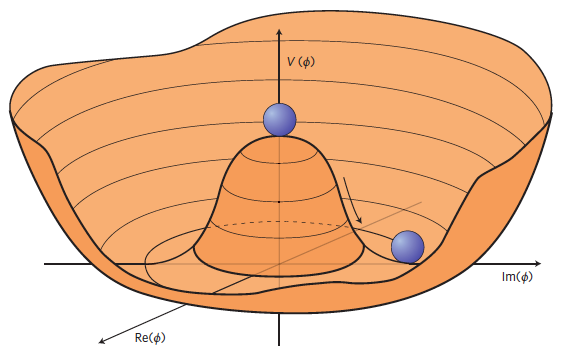
\includegraphics[width=0.7\linewidth]{Figures/higgspotential}
	\caption[Illustration of the Higgs potential for $\mu^2$ < 0]{The Higgs potential is shown as a function of the complex scalar field's real and imaginary parts. The balls illustrate that the stable vacuum state of nature is not located at $\phi$ = 0 because the symmetry at that point is spontaneously broken. Instead the stable vacuum state of nature is located somewhere along the circle of minimum potential. Reprint from \cite{Ellis:2011}}
	\label{fig:higgspotential}
\end{figure}


Writing the Lagrangian in Equation \ref{equation:higgsL} in terms of the physical $W$ and $Z$ fields and evaluating at the VEV gives 
\begin{equation}
	\begin{split}
	\mathcal{L}_{Higgs} = &\frac{1}{2}\partial_\nu h\partial^\nu h + \frac{1}{4}g_w^2W_\nu^+W^{-\nu}(v+h)^2 \\
	& + \frac{1}{8}\frac{g_w^2}{\cos^2\theta_W}Z_\nu Z^\nu (v+h)^2 - V[\frac{1}{2}(v+h)^2]
	\end{split}
\end{equation}
The $v^2$ terms give the $W$ and $Z$ boson masses and the $h^2$ term gives the mass of the Higgs boson as
\begin{eqnarray}
	M_W = \frac{1}{2}g_wv \\
	M_Z = \frac{1}{2}v\frac{g_w}{\cos\theta_W} = \frac{M_W}{\cos\theta_W} \\
	M_H = \sqrt{2}|\mu|
\end{eqnarray}
while the photon remains massless.

%We can write the Lagrangian for the weak interaction as
%\begin{equation}
%	\mathcal{L}_{QED} = \bar{\psi}(i\gamma^\mu D_\mu -m)\psi - Tr\frac{1}{8}W_{\mu \nu}W^{\mu \nu}
%	\label{equation:qedlagrangian}
%\end{equation}


%Recall that there are three vector bosons ,$W_\mu^{1,2,3}$, associated with $SU(2)_L$ and one, $B_\mu$, associated with $U(1)_Y$.  

At this point we can summarize the particle content of the SM and their allowed interactions in a way that is seen in Figure \ref{fig:smcontent}.

\begin{figure}[h]
	\centering
	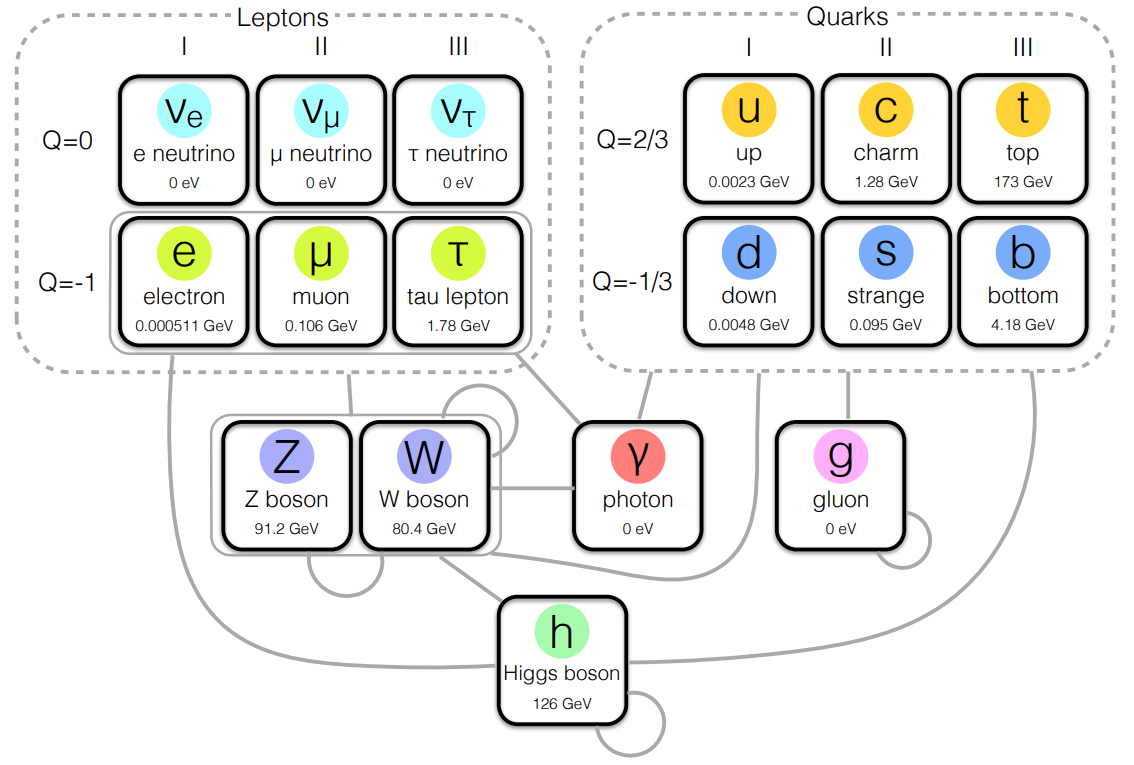
\includegraphics[width=1.0\linewidth]{Figures/SMcontent}
	\caption[Summary of content of the SM.]{Summary of particle content in the SM. Gray lines connecting groups of particles indicates allowed interactions. Self-coupling is indicated by a gray line connecting a particle to itself. The leptons and quarks are organized in columns corresponding to generation, which is specified at top, and rows corresponding to electric charge Q, which is listed to the left. Each particle's mass is listed beneath its name and symbol. It should be noted that neutrinos in the SM are still treated as massless leptons despite the fact that experimental evidence has established that at least two of the neutrinos are massive. Reprinted from \cite{Iiyama:2015nem}}
	\label{fig:smcontent}
\end{figure}


\section{Problems with the SM}